\documentclass{article}
\usepackage[letterpaper, total={7in, 8in}]{geometry}
\usepackage[utf8]{inputenc}
%\usepackage[english]{babel}
\usepackage[]{amsthm} %lets us use \begin{proof}
\usepackage[]{amsmath}
\usepackage[]{amssymb} %gives us the character \varnothing
\usepackage{mathrsfs}
\usepackage{graphicx}
\usepackage{adjustbox}
\usepackage{titlesec}
\usepackage[numbered,framed]{matlab-prettifier}
\usepackage{listings}
\usepackage[t1,OT1]{fontenc}
\usepackage{filecontents}
\usepackage{float}
\usepackage{physics}
\usepackage{csvsimple}
\usepackage{booktabs}
\usepackage{longtable}
\usepackage{algorithmicx}
\usepackage{mathtools}
\usepackage{breqn}
\usepackage{framed,color}
\usepackage{amsmath,mleftright}
\usepackage{xparse}
\usepackage{titling}
\usepackage{tabularx}
\usepackage{tikz}
\usepackage{subcaption}
\usepackage{siunitx}

\usepackage{hyperref}

\setlength{\droptitle}{-10em}   % This is your set screw

\NewDocumentCommand{\evalat}{sO{\big}mm}{%
	\IfBooleanTF{#1}
	{\mleft. #3 \mright|_{#4}}
	{#3#2|_{#4}}%
}


\DeclareMathOperator{\atantwo}{atan2}

\titleformat{\section}{\normalfont\Large\bfseries}{Section \thesection.}{1em}{}
\titleformat{\subsection}{\normalfont\large\bfseries}{\alph{subsection})}{1em}{}
\titleformat{\subsubsection}{\normalfont\bfseries}{\hspace{1em}\arabic{subsubsection})}{1em}{}

\title{Smart Products Lab 5}
\author{Tyler Morrison}
\date\today

%\lstset{
%	style              = Matlab-editor,
%	basicstyle         = \mlttfamily,
%	escapechar         = ",
%	mlshowsectionrules = true,
%	literate = {-}{-}1, % <hyphens will not show up unless you add this
%}

\lstset{
	language=C++,
%	basicstyle=\ttfamily,
	basicstyle         = \mlttfamily,
	keywordstyle=\color{blue}\ttfamily,
	stringstyle=\color{red}\ttfamily,
	commentstyle=\color{green}\ttfamily,
	morecomment=[l][\color{magenta}]{\#},
	numbers=left,
	stepnumber=1,
	frame=single
}

\renewcommand{\lstlistingname}{Program}% Listing -> Algorithm
%-------------------------------------------------------------%
%-------------------------------------------------------------%
%-------------------------------------------------------------%
\begin{document}
\maketitle
%-------------------------------------------------------------%
%--------------------------SECTION 1--------------------------%
%-------------------------------------------------------------%
\section{}
\subsection{Algorithm}
\begin{figure}[H]
	\centering
	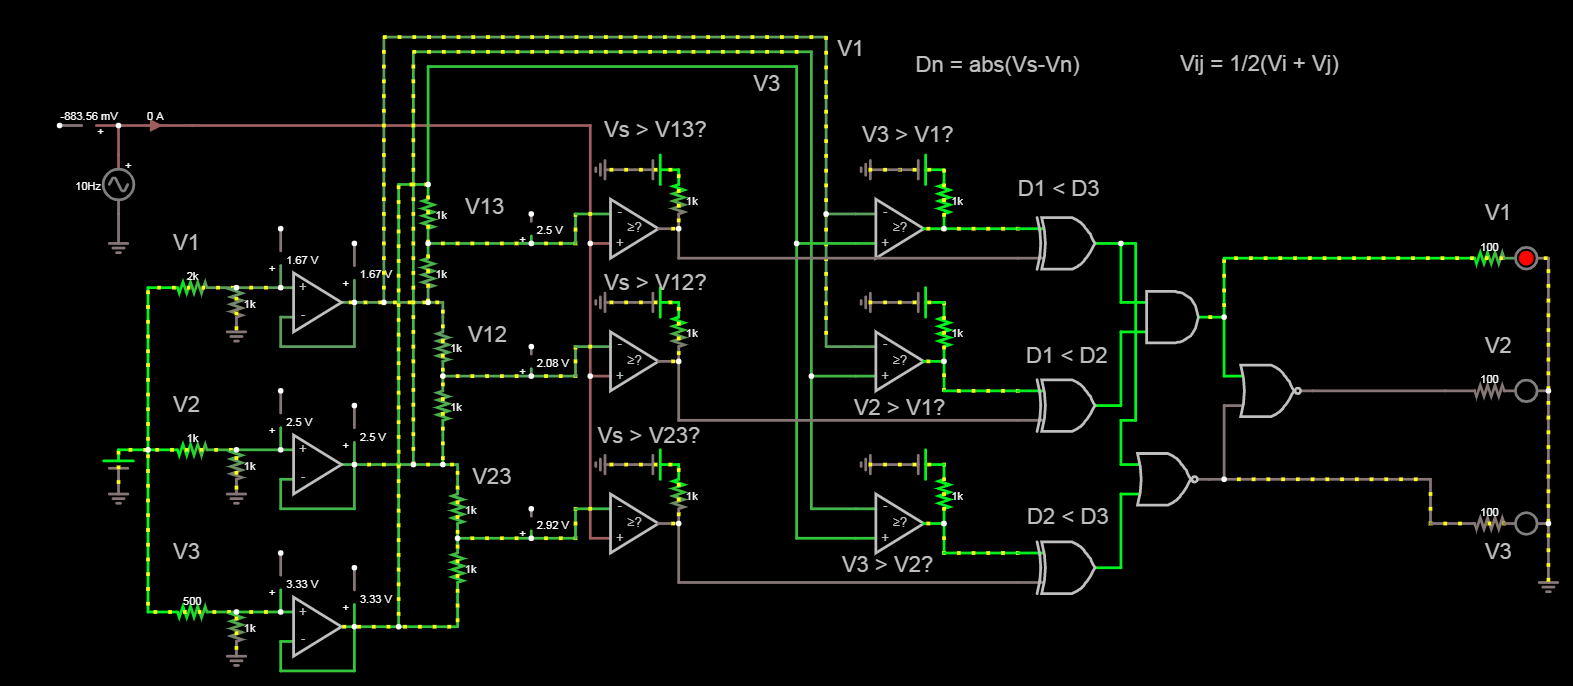
\includegraphics[keepaspectratio,width=\linewidth]{schematic.png}
	\caption{Schematic of circuit.}
\end{figure}

The op-amps at the start of our circuit isolate the supplied voltages for comparison from the rest of the circuit by providing a constant reference voltage. These are so-called ``voltage buffer amplifiers.'' The next step in our algorithm is voltage averaging which is accomplished simply by connecting two nodes of the reference voltage together with equal resistance. To understand this method consider the following equation for the averaging of $V_1$ and $V_2$: 
\begin{equation}
\frac{V_1 - V_{12}}{R} + \frac{V_2 - V_{12}}{R} = i^-
\end{equation}
Where $V_{12}$ is the average of $V_1$ and $V_2$, $R$ is the resistance between them, and $i^-$ is the current into the negative input of the comparator. However, because this current must be approximately zero because the impedance of the ideal comparator is infinite, 
\begin{equation}
V_1 - V_{12} = V_{12}- V_2
\end{equation}
and
\begin{equation}
2 V_{12} = V_1 + V_2.
\end{equation}
Without loss of generality, the same argument applies to the averages of each pair of reference voltages, and the average of each voltage can be obtained without the use of summing amplifiers.

The motivation for obtaining the averages of the reference voltages comes from converting the ``nearest voltage problem'' to its dual the ``which voltage zone'' problem. This is like converting a Delaunay triangulation to its corresponding Voroni diagram.
\begin{figure}[H]
	\centering
	\begin{tikzpicture}
	\draw[gray, thick] (-4,5) -- (-2,5); \filldraw[black] (-2,5) circle (2pt) node[anchor=west] {$V_1$};
	\draw[gray, thick] (-4,2) -- (-2,2); \filldraw[black] (-2,2) circle (2pt) node[anchor=west] {$V_3$};
	\draw[gray, thick] (-4,0) -- (-2,0); \filldraw[black] (-2,0) circle (2pt) node[anchor=west] {$V_2$};
	
	\draw[red, thick] (2,2.5) -- (4,2.5); \filldraw[red] (4,2.5) circle (2pt) node[anchor=west] {$V_{12}$};
	\draw[red, thick] (2,1.0) -- (4,1.0); \filldraw[red] (4,1.0) circle (2pt) node[anchor=west] {$V_{23}$};
	\draw[red, thick] (2,3.5) -- (4,3.5); \filldraw[red] (4,3.5) circle (2pt) node[anchor=west] {$V_{13}$};
	
	\draw[blue, thick] (2,2.8) -- (5,2.8); \filldraw[blue] (5,2.8) circle (2pt) node[anchor=west] {$V_{s}$};
	\draw[blue, thick] (-4,2.8) -- (-1.5,2.8); \filldraw[blue] (-1.5,2.8) circle (2pt) node[anchor=west] {$V_{s}$};
	
	\draw[-latex,line width=2mm] (-.5,2.5) -- (1.2,2.5);
	\end{tikzpicture}
	\caption{Converting the ``nearest voltage problem'' to its dual the ``which voltage zone'' problem.}
\end{figure}
Converting the problem in this manner allows us to avoid analog differencing operations to determine the distances between $V_s$ and the reference voltages. Instead, we simply need to know the order of the magnitudes of the reference voltages. This can be determined with comparators. Finally, we can easily determine which set of averages $V_s$ is between using comparators. For example, if $V_s > V_{12}$ and $V_{13} > V_s$, it is clear that $V_s$ is somewhere between $V_{13}$ and $V_{12}$. This allows us to convert the analog problem to a digital problem as soon as possible which limits the amount we had to mess around with analog components. We really liked this aspect of the approach.

Our six comparator outputs are simplified by a digital logic step. The following table demonstrates that by comparing $V_s$ with the average voltage, and XORing it with the comparison between the two voltage levels, we can determine which difference is larger, where the difference is $D_i = \abs{\left(V_s - V_i \right)}$.
\begin{table}[H]
	\centering
	\caption{The XOR logic comparing average voltage to the source, and the two voltages together}
	\begin{tabular}{cc|c}
		$V_s > V_{ij}$ & $V_i > V_j$ & $D_i > D_j$ \\\hline
		T & T & F \\
		T & F & T \\
		F & T & T \\
		F & F & F \\
	\end{tabular}
\end{table}

Now that we have determined $D_i > D_j$ for each combination of reference voltages, we now only need to use a truth table to devise the remaining digital logic.
%-------------------------------------------------------------%
\subsection{Truth tables}
\begin{table}[H]
	\centering
	\caption{The logic of every possible permutation of the order of differences. $V_i$ indicates that LED $i$ should be lit.}
	\begin{tabular}{ccc|lc|ccc}
		$D_3 > D_1$ & $D_2 > D_1$ & $D_3 > D_2$ & Inequalities & Smallest & $V_1$ & $V_2$ & $V_3$ \\\hline
		T & T & T & $D_3 > D_1,\quad D_2 > D_1,\quad D_3 > D_2\, \Rightarrow D_3 > D_2 > D_1$ & $D_1$ & T & F & F \\
		T & T & F & $D_3 > D_1,\quad D_2 > D_1,\quad D_2 > D_3\, \Rightarrow D_2 > D_3 > D_1$ & $D_1$ & T & F & F \\
		T & F & T & $D_3 > D_1,\quad D_1 > D_2,\quad D_3 > D_2\, \Rightarrow D_3 > D_1 > D_2$ & $D_2$ & F & T & F \\
		T & F & F & $D_3 > D_1,\quad D_1 > D_2,\quad D_2 > D_3\, \Rightarrow\;\;\quad\quad \Rightarrow\!\Leftarrow$ &  \multicolumn{4}{c}{False premise} \\
		F & T & T & $D_1 > D_3,\quad D_2 > D_1,\quad D_3 > D_2\, \Rightarrow\;\;\quad\quad \Rightarrow\!\Leftarrow$ &  \multicolumn{4}{c}{False premise} \\
		F & T & F & $D_1 > D_3,\quad D_2 > D_1,\quad D_2 > D_3\, \Rightarrow D_2 > D_1 > D_3$ & $D_3$ & F & F & T \\
		F & F & T & $D_1 > D_3,\quad D_1 > D_2,\quad D_3 > D_2\, \Rightarrow D_1 > D_3 > D_2$ & $D_2$ & F & T & F \\
		F & F & F & $D_1 > D_3,\quad D_1 > D_2,\quad D_2 > D_3\, \Rightarrow D_1 > D_2 > D_3$ & $D_3$ & F & F & T \\
	\end{tabular}
\end{table}
%\begin{table}[H]
%	\centering
%	\caption{Logic steps for valid possibilities with $(D_i > D_j) \iff D_{ij}$}
%	\begin{tabular}{ccc|cc|ccc}
%		$D_{31}$ & $D_{21}$ & $D_{32}$ & $A = D_{31} \land D_{21}$ & $B = \neg\left(D_{21} \lor D_{32}\right)$ & $V_1 = A$ & $V_2 = \neg(A \lor B)$ & $V_3 = B$ \\\hline
%		T & T & T & T & F & T & F & F \\
%		T & T & F & T & F & T & F & F \\
%		T & F & T & F & F & F & T & F \\
%		F & T & F & F & F & F & F & T \\
%		F & F & T & F & F & F & T & F \\
%		F & F & F & F & T & F & F & T \\
%	\end{tabular}
%\end{table}
%
%The above table illustrates that there is one error in the circuit. In the fourth row, a condition for $V_3$ is violated. I will explain why this mistake did not show up in testing.
%
%For the condition related to the error,
%\[D_1 > D_3,\quad D_2 > D_1,\quad D_2 > D_3\, \Rightarrow D_2 > D_1 > D_3\]

\begin{table}[H]
	\centering
	\caption{Logic steps for valid possibilities with $(D_i > D_j) \iff D_{ij}$}
	\begin{tabular}{ccc|cc|ccc}
		$D_{31}$ & $D_{21}$ & $D_{32}$ & $A = D_{31} \land D_{21}$ & $B = \neg\left(D_{32} \lor D_{31}\right)$ & $V_1 = A$ & $V_2 = \neg(A \lor B)$ & $V_3 = B$ \\\hline
		T & T & T & T & F & T & F & F \\
		T & T & F & T & F & T & F & F \\
		T & F & T & F & F & F & T & F \\
		F & T & F & F & T & F & F & T \\
		F & F & T & F & F & F & T & F \\
		F & F & F & F & T & F & F & T \\
	\end{tabular}
\end{table}
These tables demonstrate that the NOR and AND logic chips can be used to get the correct output for the circuit from the XOR chip outputs.
%-------------------------------------------------------------%
\subsection{Components}
\begin{itemize}
	\item 2 Comparator Chips -- One for comparisons to $Vs$ one for reference voltage comparison.
	\item 1 Op-Amp Chip -- For buffer amplifiers
	\item 1 XOR Chip -- For $D_i  > D_j$ logic
	\item 1 AND Chip -- For final digital logic steps
	\item 1 NOR Chip -- For final digital logic steps
\end{itemize}
%-------------------------------------------------------------%
\subsection{Other methodology}
The previous sections have more or less completely described our methodology. Averaging was the very first concept that we started with when we thought the reference voltages would be given in order. In order to accommodate arbitrary order, we added logic to the front to switch the references between positions in the original averaging circuit before using logic again at the end. In this approach, we basically found a way to collapse those two sections of logic into one and avoid switches.
%-------------------------------------------------------------%
\subsection{Incremental testing}
Most of our testing was done in the circuit simulator. In the simulator, we first confirmed we understood the op-amp functionality, the comparator functionality etc. Then, after we had our final design, we assembled the circuit, tested the logic portion manually to confirm it worked and then tested it all together. Some issues with bad connections had to be detected with the multimeter.
%-------------------------------------------------------------%
\subsection{Future attempts}
To be honest, I'm not quite sure how we could reduce the component count. There may be a way, but I can't think of anything.
%-------------------------------------------------------------%
%--------------------------SECTION 2--------------------------%
%-------------------------------------------------------------%
\section{}
\subsection{Oscilloscope output during testing}
%-------------------------------------------------------------%
%Figure of all output at frequency one
\begin{figure}[H]
	\centering
	\begin{subfigure}{.5\linewidth}
		\centering
		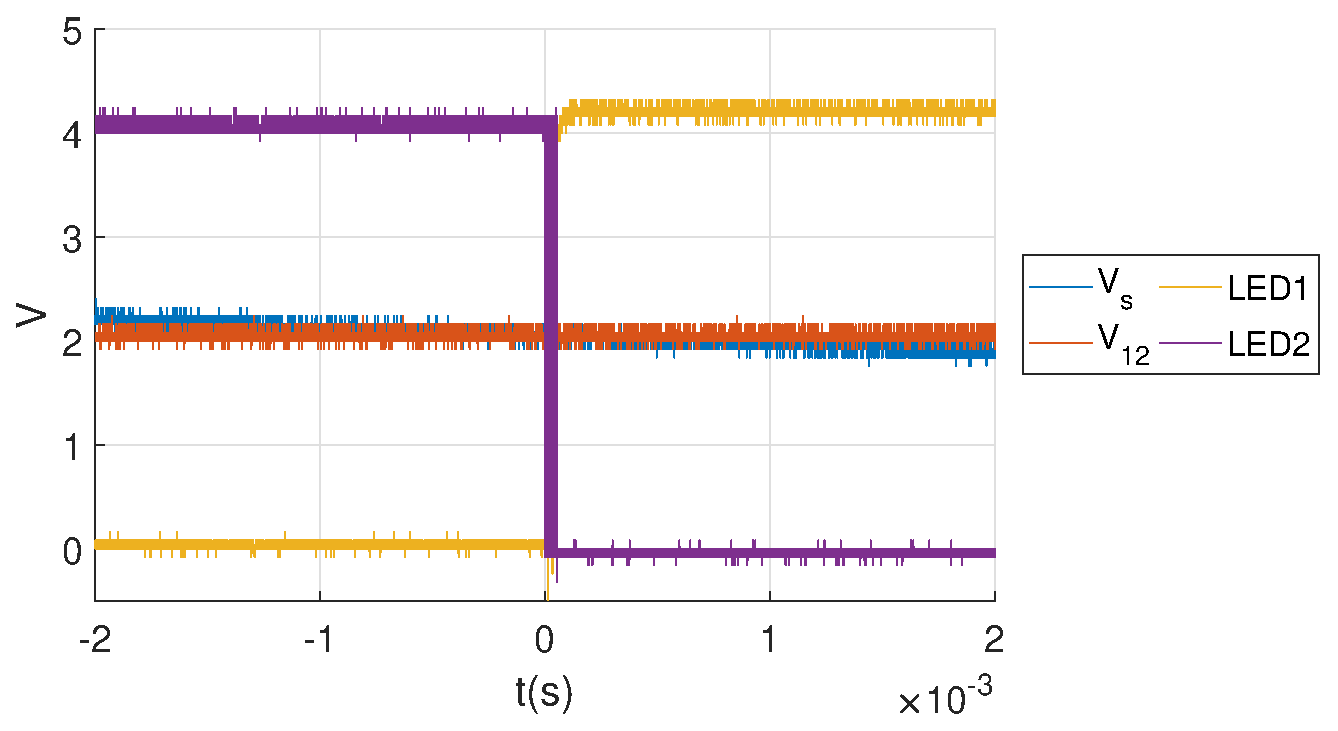
\includegraphics[keepaspectratio,width=.98\linewidth]{5hz_all.eps}
		\caption{Transition from $V_2$ to $V_1$ at 5 Hz.}
	\end{subfigure}%
	%Figure of all output at frequency two
	\begin{subfigure}{.5\linewidth}
		\centering
		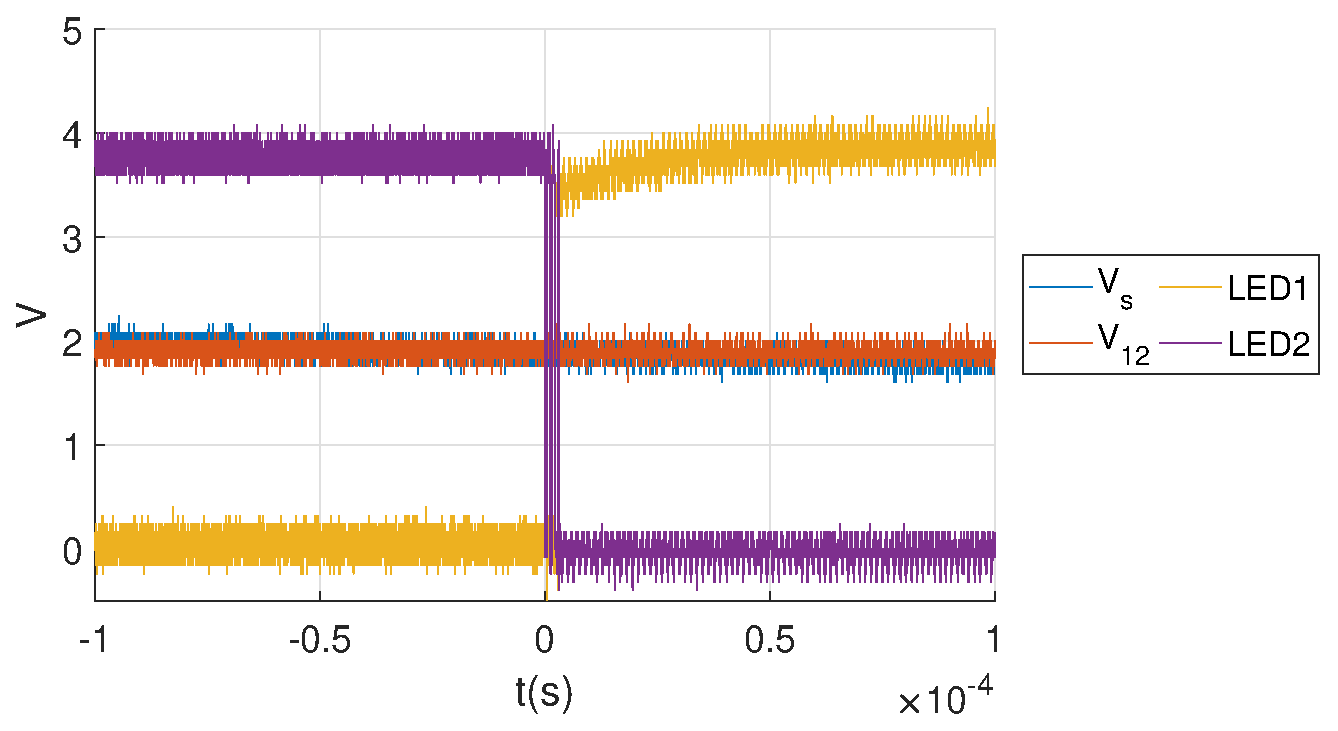
\includegraphics[keepaspectratio,width=.98\linewidth]{50hz_all.eps}
		\caption{Transition from $V_2$ to $V_1$ at 50 Hz.}
	\end{subfigure}
\caption{Circuit output with a sine wave $V_s$ falling from $V_2$ to $V_1$.}
\end{figure}
\subsection{Exercise measurements and graphics}
%-------------------------------------------------------------%
\subsubsection{Time to switch indicator lines}
% Measure the time it takes for your circuit to switch digital indictor lines. For example, starting at the instant that 𝑉𝑆 becomes closer to 𝑉𝑅1 than to 𝑉𝑅2 (as in bottom of Figure 11), how long does it take for 𝐷𝑅2 to go LOW and 𝐷𝑅1 to go HIGH. Capture this transition using analog probes.
\begin{figure}[H]
	\centering
	\begin{subfigure}{.5\linewidth}
		\centering
		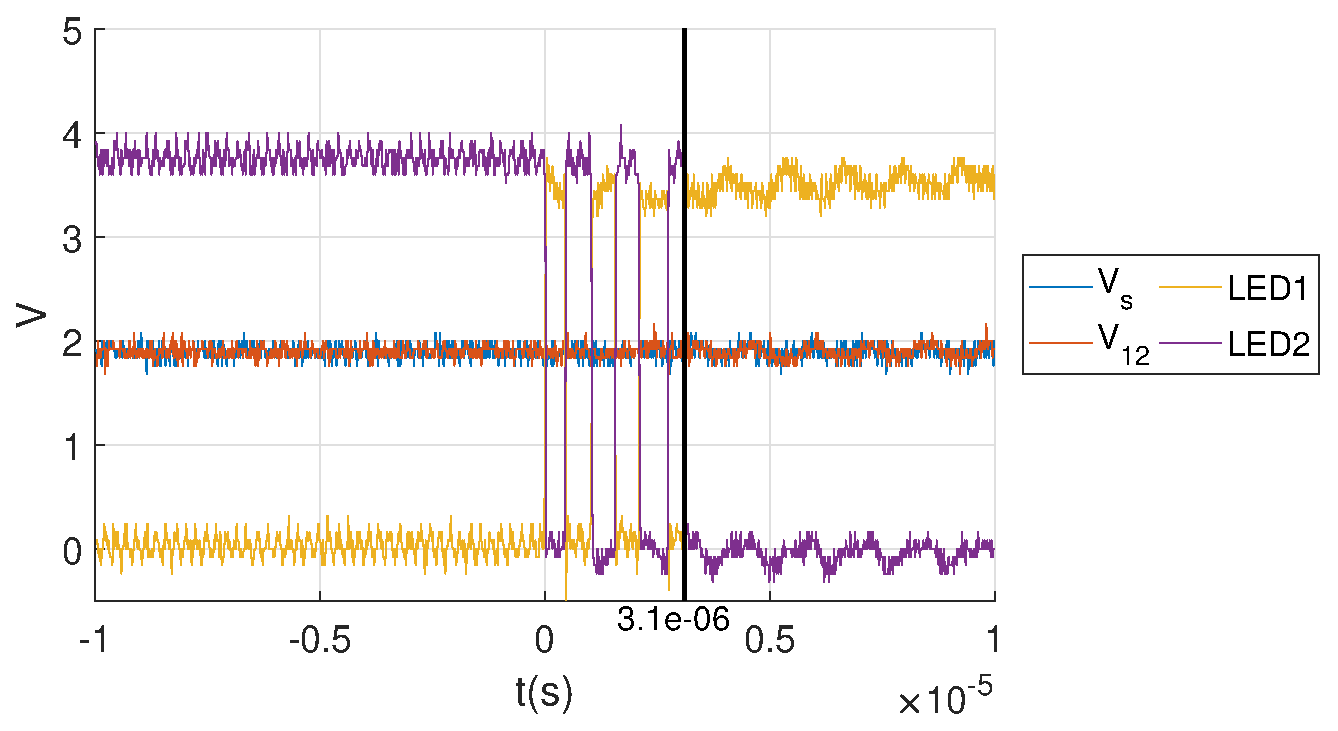
\includegraphics[keepaspectratio,width=.96\linewidth]{50hz_zoom.eps}
		\caption{Transition from $V_2$ to $V_1$ at 50 Hz.}
	\end{subfigure}%
	%Figure of all output at frequency two
	\begin{subfigure}{.5\linewidth}
		\centering
		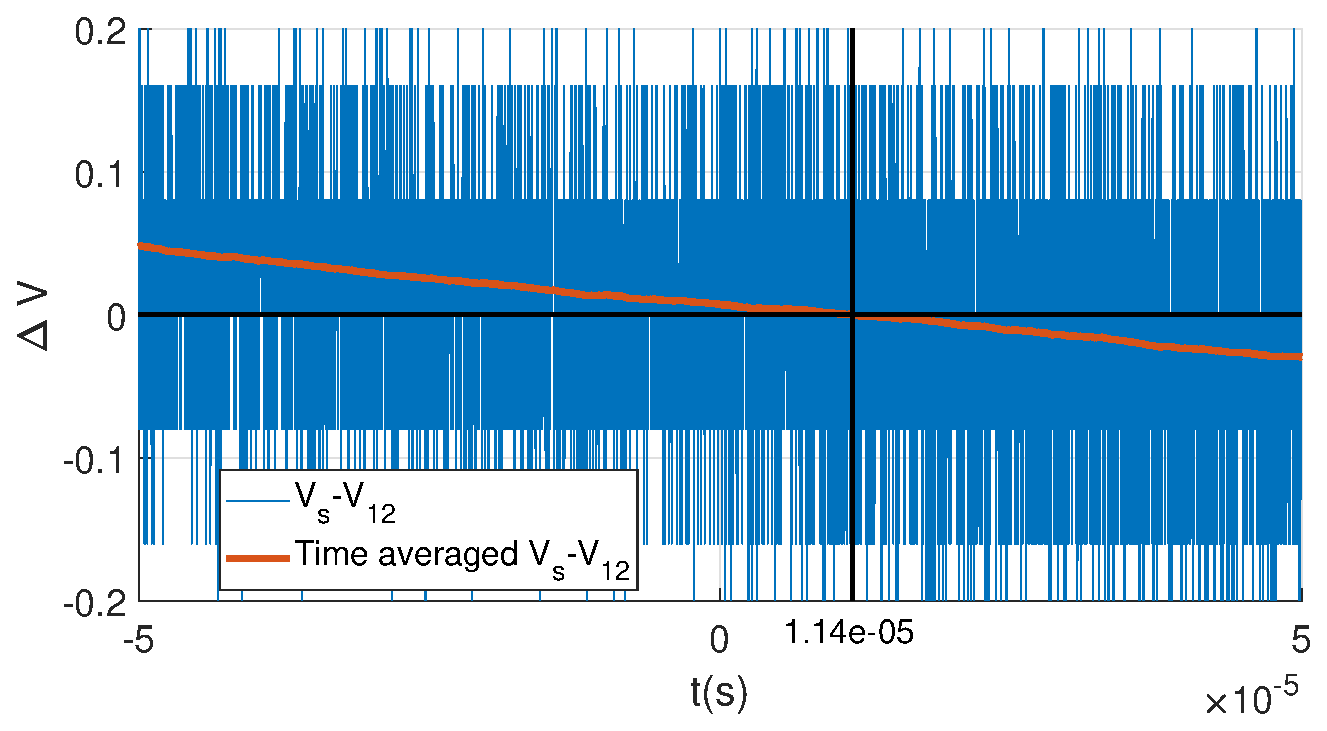
\includegraphics[keepaspectratio,width=.96\linewidth]{50hz_avg_diff.eps}
		\caption{Transition from $V_2$ to $V_1$ at 50 Hz.}
	\end{subfigure}
	\caption{Circuit output with a sine wave $V_s$ falling from $V_2$ to $V_1$.}
\end{figure}
The above figures show the time at which LED1 finally stays high and the time at which $V_s$ crosses the $V_{12}$ average. These times are actually in the wrong order meaning that the noise in the difference between the voltage levels is too much for us to measure an accurate crossing time to measure the lag. For all intents and purposes it seems instantaneous. However, in hindsight, we should increase the source frequency to narrow the window of time of crossing and better determine the delay time. In this case, all we know is that it is less than $\SI{3}{\micro\second}$.
\subsubsection{Minimum frequency for simultaneous illumination}
% Run your circuit through several frequencies of a sinusoidal signal. What is the minimum frequency of the signal line which causes multiple LEDs to illuminate at once? Probe and capture the digital indictor lines and describe the signals that are being produced. Explain why multiple LEDs are illuminated. What other microcontroller process causes this type of phenomena?
While increasing the frequency, at around 14 Hz it was hard to tell whether the LEDs were blinking in unison on sequentially. By around 43 Hz, all three LEDs seemed to be constantly illuminated. LED2, configured for the middle voltage seemed to go steady first and when all the LEDs were steady appeared the dimmest.

The appearance of LED2 is explained by the fact that because it is the middle voltage, for our source sine wave, it is active for a shorter period of time. All three LEDs appear to be illuminated because their blinking exceeds the rate that human eyes can detect. This is, in effect, how lots of modern light sources work.

The fact that when the voltages get near a transition point, noise in the system causes high frequency switching only increases this effect, making it seem as if two lights are illuminated at once because they are switching on and off at the noise frequency which is much higher than the source frequency.

\begin{figure}[H]
	\centering
	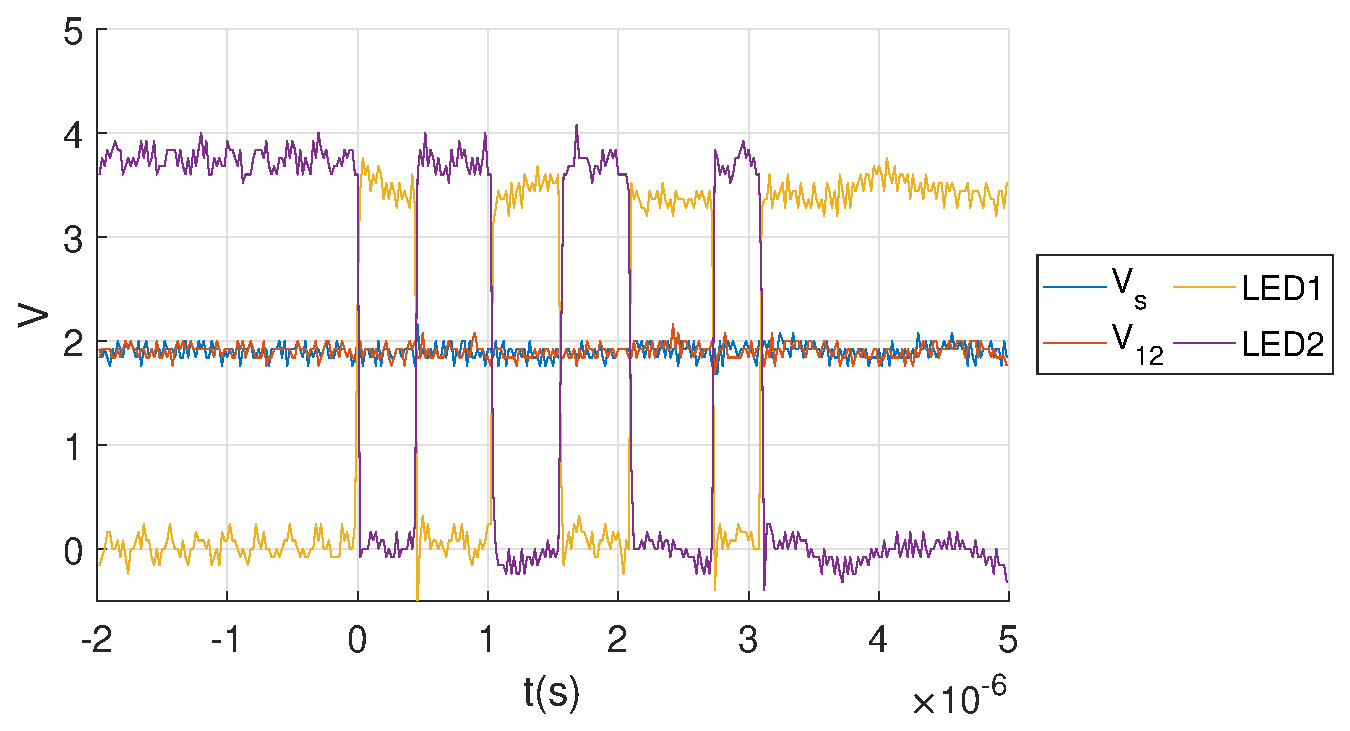
\includegraphics[keepaspectratio,width=.8\linewidth]{50hz_zoom2.eps}
	\caption{High frequency switching on the digital output line due to noise near the transition point.}
\end{figure}

\subsection{Picture}
\begin{figure}[H]
	\centering
	\includegraphics[keepaspectratio,width=.7\linewidth]{circuit_pic.jpg}
	\caption{Photo of completed circuit.}
\end{figure}
%-------------------------------------------------------------%
%-------------------------------------------------------------%
%-------------------------------------------------------------%
\end{document}